\documentclass[12t, a4paper]{article}
\usepackage{CJKutf8}
\usepackage[left=2cm, right=2cm, top=3cm, bottom=2.5cm]{geometry}
\usepackage[nodayofweek,level]{datetime}
\usepackage{comment}

%..This section controls the header-footer layout of the document
\usepackage{fancyhdr}
\pagestyle{fancy}
\lhead{Computer Architecture (NTU CSIE, Fall 2017)}
\chead{}
\rhead{Homework \#4}
\renewcommand{\headrulewidth}{0.4pt}

%..This section controls the title layout
\title{\vspace{-4ex}\bf{\LARGE{Homework \#4}}} 
\author{資工三\space B04902009\space蕭千惠} % \footnote{blablabla} 
\date{\vspace{-2ex}\today\vspace{-4ex}}
%{\formatdate{21}{2}{2017}}

%.. code
\usepackage{listings}
\lstset{language=Verilog}

\makeatother

%.. Customize section numbering
% \renewcommand\thesubsection{(\arabic{subsection})}
\usepackage{color}

%.. Insert graph
\usepackage{graphicx}
% \includegraphics[width=\textwidth, height=10cm, keepaspectratio=true]{pic.jpg}

%.. indent
\usepackage{indentfirst}
\setlength{\parindent}{2em}

%.. hyperlink / url
\usepackage[hyphens]{url}
\usepackage{hyperref}
\hypersetup{
    colorlinks=true,
    linkcolor=blue,
    filecolor=magenta,      
    urlcolor=blue,
}
\urlstyle{same}
%%\url{url}
%%\herf{url}{words to show}

%.. change font size
\usepackage{type1cm}

%.. change enumerate label
\usepackage{enumitem}
%%\begin{enumerate}[label=(\alph*)]  //(a) (b) (c)
%%\begin{enumerate}[label=(\Alph*)]  //(A) (B) (C)
%%\begin{enumerate}[label=(\roman*)] //(i) (ii) (iii`')

%.. define tab
\newcommand\tab[1][1cm]{\hspace*{#1}}



%.. Content
\begin{document}
	\begin{CJK}{UTF8}{bkai}
	\maketitle\thispagestyle{fancy}
	\fontsize{12pt}{16pt} \selectfont
	% \noindent
	\section{Coding Environment}
		Apple: OS X EL Capitan

	\section{Module implementation explanation}
		\subsection{CPU}
			畫出 data path 來釐清誰的 output 會連接到誰的 input \\
			\centerline{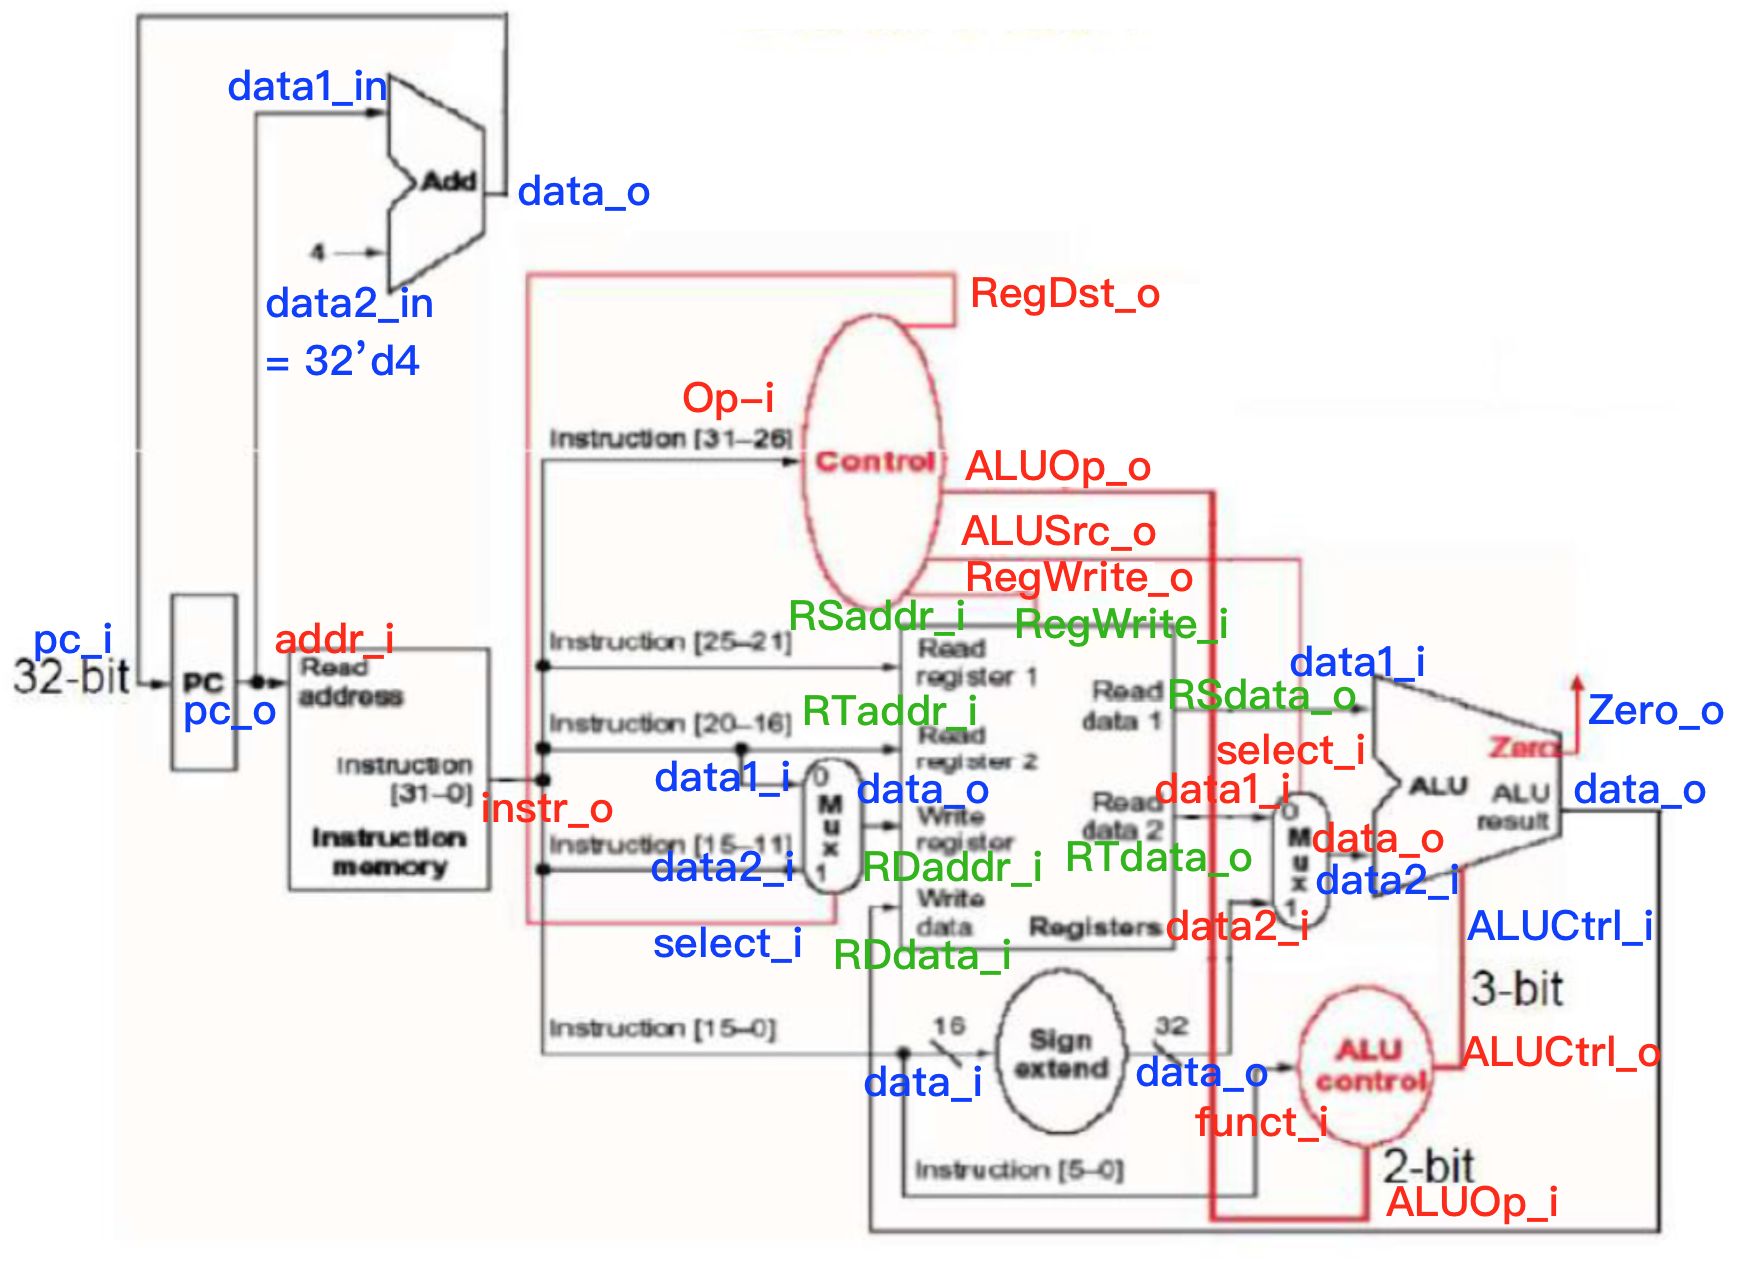
\includegraphics[width=15cm, keepaspectratio=true]{data_path.png}} \par
		
		\subsection{Adder}
			\begin{verbatim}
			   data_o = data1_in + data2_in
			\end{verbatim}	
		
		\subsection{Control}
			依照下表判斷 Opcode 對應到哪個指令,並依照該指令輸出對應的 Control Signal \par \vspace{0.2cm}
			\begin{tabular}[c]{|c|c|c|c|c|c|}
			\hline
				Instruction	& Opcode & ALUOp & RegDst & ALUSrc & RegWrite \\
				&(Input)&(Output)&(Output)&(Output)&(Output)\\
			\hline
				R-type & 000000(0x00) & 11(Rtype) & 1 & 0 & 1 \\
			\hline
				addi & 001000(0x08) & 00(add) & 0 & 1 & 1 \\
			\hline
			\end{tabular}

		\subsection{ALU}
			依照下表的 ALU control 值決定要執行哪一種運算 \par \vspace{0.2cm}
			\begin{tabular}[c]{|c|c|c|c|c|c|}
			\hline
							&and	&or		&add 	&sub 	&mul \\
			\hline
				ALU control &000 	&001 	&010 	&110 	&101 \\
			\hline
			\end{tabular}  \vspace{0.1cm}
			\begin{verbatim}
			   data_o = (ALUCtrl_i == 3'b000)?	data1_i & data2_i :
			            (ALUCtrl_i == 3'b001)?	data1_i | data2_i :
			            (ALUCtrl_i == 3'b010)?	data1_i + data2_i :
			            (ALUCtrl_i == 3'b110)?	data1_i - data2_i :
			            (ALUCtrl_i == 3'b101)?	data1_i * data2_i :
			            32'd0;
			\end{verbatim}
			
		\subsection{ALU\_Control}
			依照下表的 Opcode 和 function code 決定輸出的 ALU ctrl 為何 \par
			{\bf \large R-type (Opcode=0x00, ALUOp=11)} \par  \vspace{0.2em}
			\begin{tabular}[c]{|c|c|c|c|c|}
			\hline
				Instruction	&Opcode			&ALUOp		&Func\_code		&ALU\_ctrl \\
			\hline
				add			&000000(0x00)	&11(Rtype)	&100000(0x20)	&010 \\
			\hline
				sub			&000000(0x00)	&11(Rtype)	&100010(0x22)	&110 \\
			\hline
				and			&000000(0x00)	&11(Rtype)	&100100(0x24)	&000 \\
			\hline
				or			&000000(0x00)	&11(Rtype)	&100101(0x25)	&001 \\
			\hline
				mul			&000000(0x00)	&11(Rtype)	&011000(0x18)	&101(Self\_defined) \\
			\hline
			\end{tabular}  \par \vspace{0.4em}
			{\bf \large I-type (no Func\_code)} \par  \vspace{0.3em}
			\begin{tabular}[c]{|c|c|c|c|c|}
			\hline
				Instruction	&Opcode			&ALUOp		&Func\_code	&ALU\_ctrl \\
			\hline
				addi		&001000(0x08)	&00(add)	&X			&010 \\
			\hline
			\end{tabular} \par \vspace{0.1cm}
			
			\begin{verbatim}
			   assign ALUCtrl_o = (ALUOp_i == 2'b00)?                     3'b010 :   // addi
			                      (ALUOp_i == 2'b11 && funct_i == 6'h20)?	3'b010 :   // add
			                      (ALUOp_i == 2'b11 && funct_i == 6'h22)?	3'b110 :   // sub
			                      (ALUOp_i == 2'b11 && funct_i == 6'h24)?	3'b000 :   // and
			                      (ALUOp_i == 2'b11 && funct_i == 6'h25)?	3'b001 :   // or
			                      (ALUOp_i == 2'b11 && funct_i == 6'h18)?	3'b101 :   // mul
			                      3'b000;
			\end{verbatim}

		\subsection{MUX5 \& MUX32}
			如果 select 是 1 (True),輸出 data1,反之則輸出 data2 \par
			\begin{verbatim}
			   data_o = (select_i == 1'b0)?	data1_i : data2_i;
			\end{verbatim}

		\subsection{Sign\_Extend}
			輸出為 32 bits,而輸入為 16 bits。 \par
			Sign extension 要做的就是把輸入的 Most significant bit 複製到不足的 16 bits 上。\par
			\begin{verbatim}
			   data_o = {{16{data_i[15]}}, data_i};	
			\end{verbatim}
	
	\clearpage
	\end{CJK}
\end{document}